\documentclass[tikz,border=4pt]{standalone}
\usepackage{tikz}
\usetikzlibrary{patterns,arrows.meta}
\definecolor{nebula}{HTML}{6366F1}
\definecolor{spark}{HTML}{14B8A6}
\begin{document}
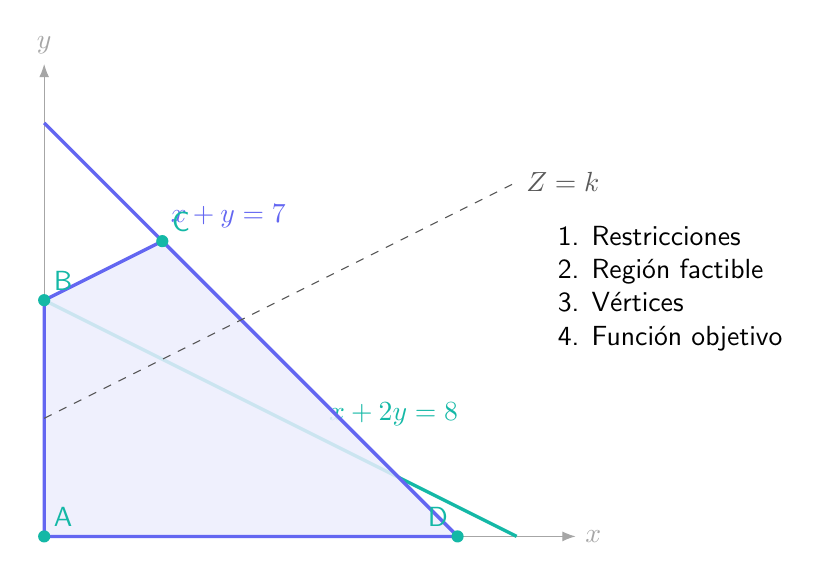
\begin{tikzpicture}[x=.75cm,y=.75cm,font=\sffamily,>=Latex]
  \draw[->,gray!70] (0,0)--(9,0) node[right] {$x$};
  \draw[->,gray!70] (0,0)--(0,8) node[above] {$y$};
  \draw[very thick,nebula] (0,7)--(7,0) node[pos=.28,above right] {$x+y=7$};
  \draw[very thick,spark] (0,4)--(8,0) node[pos=.58,above right] {$x+2y=8$};
  \fill[nebula!12,opacity=.85] (0,0)--(0,4)--(2,5)--(7,0)--cycle;
  \draw[very thick,nebula] (0,0)--(0,4)--(2,5)--(7,0)--cycle;
  \foreach \p/\lab in {(0,0)/A,(0,4)/B,(2,5)/C}{\fill[spark] \p circle(2.2pt) node[above right] {\lab};}
  \fill[spark] (7,0) circle(2.2pt) node[above left] {D};
  \draw[dashed,black!65] (0,2)--(8,6) node[right] {$Z=k$};
  \node[align=left] at (10.6,4.2) {1. Restricciones\\2. Regi\'on factible\\3. V\'ertices\\4. Funci\'on objetivo};
\end{tikzpicture}
\end{document}
